\documentclass[10pt,letterpaper]{article} 
\usepackage{tikz}
\usepackage{toolsper}
%\usepackage{graphicx}‎‎
%\usefonttheme{serif}‎
%\usepackage{ptext}‎
%\usepackage{xepersian}
%\settextfont{B Nazanin}
\usepackage{lipsum}
\setlength{\parindent}{0pt}
%\usepackage{enumitem}
%\setlist[enumerate,1]{label=(\arabic*)}
\newcommand{\pf}{$\blacksquare$}
\newcommand{\EX}{\Bbb E}
\newcommand{\nl}{\newline\newline}
\setlength{\parskip}{1em}

\usepackage{amsmath}
\usepackage{accents}
\newlength{\dhatheight}
\newcommand{\doublehat}[1]{%
    \settoheight{\dhatheight}{\ensuremath{\hat{#1}}}%
    \addtolength{\dhatheight}{-0.35ex}%
    \hat{\vphantom{\rule{1pt}{\dhatheight}}%
    \smash{\hat{#1}}}}

\newcounter{QuestionNumber}
\setcounter{QuestionNumber}{1}

\newcommand{\Q}{
\textbf{
سوال \theQuestionNumber)
}
\stepcounter{QuestionNumber}
}

\newcommand{\fig}[3]{
\begin{figure}[h!]
#1
\caption{#2}
\label{#3}
\end{figure}
}

\newcommand{\subfig}[3]{
\begin{subfigure}{#3}
#1
\caption{#2}
\end{subfigure}
}
%\newcommand{\pic}[2]{
%\begin{center}
%\includegraphics[width=#2]{#1}
%\end{center}
%}
\begin{document}
\Large
\begin{center}
به نام زیبایی

تمرینات سری یازدهم سیگنال ها و سیستم ها
\hl
\end{center}
\Q
(مفهومی)

الف) چرا ناحیه‌ی همگرایی تبدیل لاپلاس نمی تواند شامل قطب باشد؟

ب) اگر سیگنال های $x(t)$ و $y(t)$ دارای تبدیل های لاپلاس 
$
X(s)
$
 و
$
Y(s)
$
 باشند، تحت چه شرایطی سیگنال 
$
z(t)=x(t)+y(t)
$
 دارای تبدیل لاپلاس است؟ (راهنمایی: به نواحی همگرایی توجه کنید.)

\Q

تبدیل لاپلاس هر یک از سیگنال های زیر را به همراه نواحی همگرایی و نمودار صفر-قطب به  دست آورید. مواردی را که تبدیل لاپلاس ندارند، با استدلال پیدا کنید.

الف)
$
x(t)=e^{-2t}u(t)+e^{-3t}u(t)
$

ب)
$
x(t)=e^tu(-t)+u(t)
$

پ)
$
x(t)=e^t\sin tu(-t)+e^{2t}u(t)
$

ت)
$
x(t)=e^{t}u(-t)+e^{-t}u(t)
$

ث) 
$
x(t)=te^{-|t|}
$

\Q

برای هر یک از تبدیل لاپلاس های زیر، سیگنال حوزه زمان را با توجه به ناحیه همگرایی داده شده به دست آورید.

الف)
$
X(s)={1\over s^2+9}\quad,\quad \Re\{s\}>0
$

ب)
$
X(s)={s\over s^2+9}\quad,\quad \Re\{s\}<0
$

پ) 
$
X(s)={s+1\over s^2+5s+6}\quad,\quad -3<\Re\{s\}<-2
$

ت) 
$
X(s)={s^2-s+1\over (s+1)^2(s+2)}\quad,\quad \Re\{s\}<-2
$

\Q

برای هر یک از گزاره های زیر برای سیگنال $x(t)$ و هر یک از نمودار های صفر-قطب زیر، ناحیه‌ی همگرایی را تعیین کنید (16 حالت مختلف وجود دارد).

الف)
$
x(t)e^{-3t}
$
مطلقا انتگرال پذیر است.

ب)
$
x(t)*[e^{-t}u(t)]
$
مطلقا انتگرال پذیر است.

پ)
$
x(t)=0\quad,\quad t>1
$

ت)
$
x(t)=0\quad,\quad t<-1
$

\begin{figure}[h!]
\centering
\begin{subfigure}{0.49\textwidth}
\includegraphics[width=80mm]{PS11_Q3_1.eps}
\caption{شکل 1}
\end{subfigure}
%%%%%%%%%%%%%%%%
\begin{subfigure}{0.49\textwidth}
\includegraphics[width=80mm]{PS11_Q3_2.eps}
\caption{شکل 2}
\end{subfigure}
%%%%%%%%%%%%%%%%
\begin{subfigure}{0.49\textwidth}
\includegraphics[width=80mm]{PS11_Q3_3.eps}
\caption{شکل 3}
\end{subfigure}
%%%%%%%%%%%%%%%%
\begin{subfigure}{0.49\textwidth}
\includegraphics[width=80mm]{PS11_Q3_4.eps}
\caption{شکل 4}
\end{subfigure}
%%%%%%%%%%%%%%%%
\end{figure}

\Q

حقایق زیر در مورد سیگنال $x(t)$ با تبدیل لاپلاس $X(s)$ به ما داده شده است:

الف)
$
X(s)
$
 دقیقا دو قطب دارد.

ب)
$
X(s)
$
 هیچ صفر محدودی ندارد (می تواند در $\pm\infty$ صفر داشته باشد).

پ) 
$
X(s)
$
 یک قطب در 
$
s=-1+j
$
 دارد.

ت)
$
e^{2t}x(t)
$
 مطلقا انتگرال پذیر نیست.

ث) 
$
X(0)=8
$

در اینصورت
$
X(s)
$
 و ناحیه همگرایی آن را بیابید.

\Q

فرض کنید اطلاعات زیر در مورد یک سیستم پایدار و علی با پاسخ ضربه‌ی $h(t)$ و پاسخ فرکانسی $H(s)$ به ما داده شده است:

1. $H(1)=0.2$

2.
اگر ورودی 
$
u(t)
$
باشد، خروجی مطلقا انتگرال پذیر است.

2.
اگر ورودی 
$
tu(t)
$
باشد، خروجی مطلقا انتگرال پذیر نیست.

4.
سیگنال 
$
{d^2h(t)\over dt^2}+2{dh(t)\over dt}+2h(t)
$
 دارای دوره‌ی محدود است.

5.
$
H(s)
$
دقیقا یک صفر در 
$
\infty
$
دارد.

در این صورت، 
$
H(s)
$
 و ناحیه همگرایی آن را بیابید.

\Q

برای هر یک از نمودار های صفر-قطب زیر، اندازه ی تبدیل فوریه را به صورت هندسی (و تقریبی) رسم کنید.

\begin{figure}[h!]
\centering
\begin{subfigure}{0.49\textwidth}
\includegraphics[width=80mm]{PS11_Q7_1.eps}
\caption{شکل 1}
\end{subfigure}
%%%%%%%%%%%%%%%%
\begin{subfigure}{0.49\textwidth}
\includegraphics[width=80mm]{PS11_Q7_2.eps}
\caption{شکل 2}
\end{subfigure}
%%%%%%%%%%%%%%%%
\begin{subfigure}{0.49\textwidth}
\includegraphics[width=80mm]{PS11_Q7_3.eps}
\caption{شکل 3}
\end{subfigure}
%%%%%%%%%%%%%%%%
\begin{subfigure}{0.49\textwidth}
\includegraphics[width=80mm]{PS11_Q7_4.eps}
\caption{شکل 4}
\end{subfigure}
%%%%%%%%%%%%%%%%
\end{figure}
\begin{figure}[h!]
\ContinuedFloat
\centering
\begin{subfigure}{0.49\textwidth}
\includegraphics[width=80mm]{PS11_Q7_5.eps}
\caption{شکل 5}
\end{subfigure}
%%%%%%%%%%%%%%%%
\begin{subfigure}{0.49\textwidth}
\includegraphics[width=80mm]{PS11_Q7_6.eps}
\caption{شکل 6}
\end{subfigure}
%%%%%%%%%%%%%%%%
%\begin{subfigure}{0.49\textwidth}
%\includegraphics[width=80mm]{PS11_Q7_3.eps}
%\caption{شکل 3}
%\end{subfigure}
%%%%%%%%%%%%%%%%%
%\begin{subfigure}{0.49\textwidth}
%\includegraphics[width=80mm]{PS11_Q7_4.eps}
%\caption{شکل 4}
%\end{subfigure}
%%%%%%%%%%%%%%%%
\end{figure}

\newpage
\Q

سیستم LTI ای با رابطه‌ی ورودی-خروجی زیر داده شده است:
$$
{d^2y(t)\over dt^2}-{dy(t)\over dt}-2y(t)=x(t)
$$
فرض کنید پاسخ ضربه‌ی آن
$
h(t)
$
 با تبدیل لاپلاس 
$
H(s)
$
باشد.

الف)
$
H(s)
$
 را به صورت حاصل تقسیم دو چندجمله ای گویا بر حسب $s$ بنویسید.

ب) 
$
h(t)
$
 را برای حالت های زیر بیابید:

1. سیستم پایدار باشد.

2. سیستم علی باشد.

3. سیستم نه پایدار و نه علی باشد.

\Q
(خواص تبدیل لاپلاس)

اگر $x(t)$ دارای تبدیل لاپلاس $X(s)$ با ناحیه همگرایی ROC=R باشد، نشان دهید:

1.
\qn{
x^*(t)\iff X^*(s^*)\quad,\quad \text{ROC}=R
}{}

2.
\qn{
{d\over dt}x(t)\iff sX(s)\quad,\quad \text{ROC}=\text{حداقل R}
}{}

3.
\qn{
-tx(t)\iff {d\over ds}X(s)\quad,\quad \text{ROC}=R
}{}

4.
\qn{
\int_{-\infty}^tx(\tau)d\tau\iff {1\over s}X(s)\quad,\quad \text{ROC}=
R\cap\{\Re\{s\}>0\}
\text{ حداقل }
}{}

\Q

فرض کنید سیستم پایدار و علی با پاسخ ضربه‌ی $h(t)$ با تبدیل لاپلاس گویا داده شده است.

الف) آیا سیستمی با پاسخ ضربه‌ی 
$
{dh(t)\over dt}
$
 همواره پایدار و علی است؟

ب) آیا سیستمی با پاسخ ضربه‌ی 
$
\int_{-\infty}^{t}h(\tau)d\tau
$
 همواره ناپایدار و علی است؟

\Q
(امتیازی)

اگر سیگنال 
$
x(t)
$
 به صورت زیر داده شده باشد:
$$
x(t)=\sum_{n=0}^{\infty}e^{-nT}\delta(t-nT)
$$
الف) 
$
X(s)
$
 را به همراه ناحیه همگرایی آن به دست آورید.

ب) نمودار صفر-قطب 
$
X(s)
$
 را رسم کنید.

پ) به کمک تعبیر هندسی نمودار صفر-قطب، نتیجه بگیرید تبدیل فوریه‌ی $x(t)$، 
$
X(j\omega)
$
، متناوب است.

%\Q
%
%فرض کنید 
%$
%X(e^{j\omega})
%$
% تبدیل فوریه‌ی سیگنال زیر باشد:
%%\begin{figure}[h!]
%%\centering
%%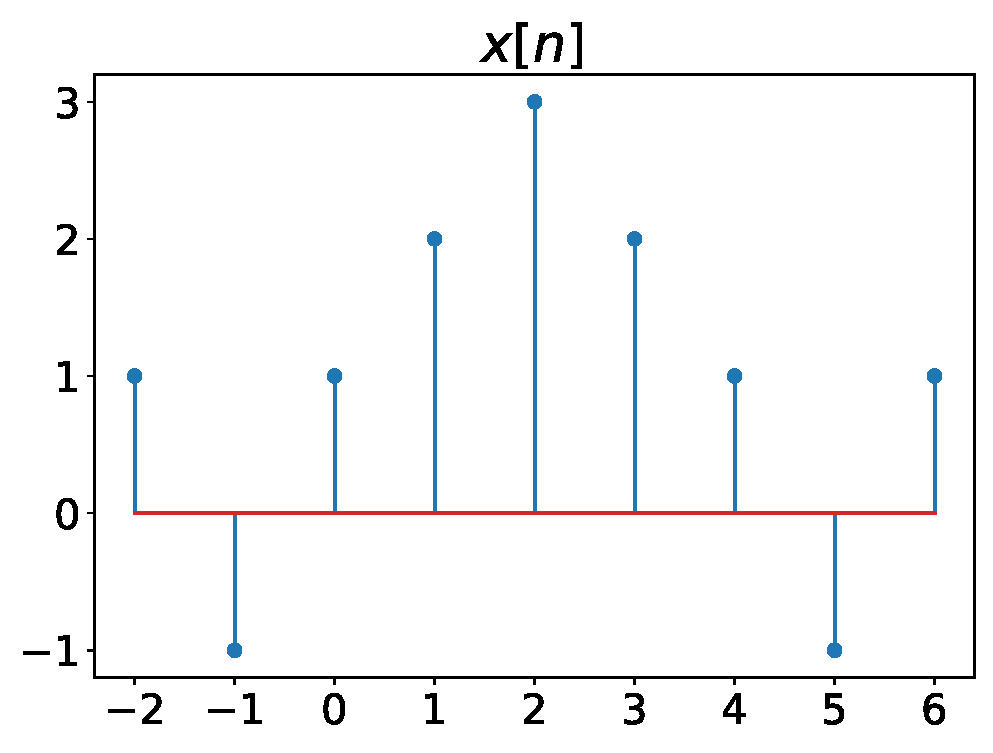
\includegraphics[width=90mm]{PS10_Q3.eps}
%%\end{figure}
%
%در این صورت، موارد زیر را به کمک خواص تبدیل فوریه بیابید:
%
%الف)
%$
%X(e^{j0})
%$
%
%ب)
%$
%\measuredangle X(e^{j\omega})
%$
%
%پ)
%$
%\int_{-\pi}^{\pi} X(e^{j\omega})d\omega
%$
%
%ت)
%$
%X(e^{j\pi})
%$
%
%ث)
%$
%\int_{-\pi}^{\pi} |X(e^{j\omega})|^2d\omega
%$
%
%ج)
%$
%\int_{-\pi}^{\pi} \left|{dX(e^{j\omega})\over d\omega}\right|^2d\omega
%$
%
%چ) سیگنالی که تبدیل فوریه‌ی آن 
%$
%\Re\{X(e^{j\omega})\}
%$
% باشد.
%
%\Q
%
%اگر $x[n]$ دارای تبدیل فوریه‌ی 
%$
%X(e^{j\omega})
%$
% باشد، تبدیل فوریه‌ی سیگنال های زیر را بر حسب
%$
%X(e^{j\omega})
%$
%بنویسید.
%
%الف)
%$
%y[n]=x[-1-n]+x[1-n]
%$
%
%ب)
%$
%y[n]={x^*[-n]+x[n]\over 2}
%$
%
%پ)
%$
%y[n]=(n-1)^2x[n]
%$
%
%\Q
%
%فرض کنید اطلاعات زیر در خصوص یک سیستم LTI با پاسخ فرکانسی 
%$
%H(e^{j\omega})
%$
% و پاسخ ضربه‌ی 
%$
%h[n]
%$
% داده شده است:
%
%$\blacksquare$
%$({1\over 4})^u[n]\longrightarrow g[n]$ 
%که در آن 
%$
%g[n]=0
%$
%اگر $n<0$ یا $n\ge 2$
%
%$\blacksquare$
%$H(e^{j{\pi\over 2}})=1$
%
%$\blacksquare$
%$H(e^{j\omega})=H(e^{j(\omega-\pi)})$
%
%در این صورت 
%$
%h[n]
%$
% را بیابید.
%
%\Q
%
%سیستم LTI ای را در نظر بگیرید که از سری کردن دو سیستم زیر به دست آمده است:
%$$
%H_1(e^{j\omega})={2-e^{-j\omega}\over 1+{1\over 2}e^{-j\omega}}
%$$
%و
%$$
%H_1(e^{j\omega})={1\over 1-{1\over 2}e^{-j\omega}+{1\over 4}e^{-j2\omega}}
%$$
%در این صورت:
%
%الف)
%معادله‌ی تفاضلی سیستم کلی را بیابید.
%
%ب) پاسخ ضربه‌ی سیستم کلی را بیابید.
%
%\Q
%
%یک سیستم LTI، دارای معادله تفاضلی زیر است:
%$$
%y[n]-ay[n-1]=bx[n]+x[n-1]
%$$
%که در آن، 
%$
%a\in \Bbb R
%$
% و 
%$
%|a|<1
%$.
%
%الف) مقدار $b$ را چنان بیابید به گونه ای که
%$$
%|H(e^{j\omega})|=1\quad,\quad \text{ برای هر $\omega$}
%$$
% به چنین سیستمی تمام گذر می گویند؛ زیرا هیچ تضعیفی روی دامنه‌ی فرکانسی سیگنال ورودی اعمال نمی‌کند. از مقدار $b$ به دست آمده در این قسمت، برای بخش های بعدی بهره ببرید.
%
%ب) به طور تقریبی، 
%$
%\measuredangle H(e^{j\omega})
%$
% را به ازای
%$
%a={1\over 2}
%$
% رسم کنید.
%
%پ) به طور تقریبی، 
%$
%\measuredangle H(e^{j\omega})
%$
% را به ازای
%$
%a=-{1\over 2}
%$
% رسم کنید.
%
%ت)
% خروجی این سیستم را به ورودی 
%$
%x[n]=({1\over 2})^nu[n]
%$
% زمانی که
%$
%a=-{1\over 2}
%$
% به دست آورده و رسم کنید. 
%
%از این مثال می توان دید که یه اثر غیرخطی در فاز در مقایسه با شیفت فاز خطی، می تواند اثر متفاوتی بر حوزه‌ی زمان سیگنال بر جا گذارد.
%
%\Q
%
%یک سیستم LTI با پاسخ ضربه‌ی $h[n]$ و پاسخ فرکانسی 
%$
%H(e^{j\omega})
%$
% دارای این خاصیت است که برای هر 
%$
%-\pi\le \omega_0\le \pi
%$
%:
%$$
%\cos \omega_0 n\longrightarrow \omega_0\cos \omega_0n
%$$
%در این صورت:
%
%الف)
%$
%H(e^{j\omega})
%$
% را بیابید.
%
%ب)
%$
%h[n]
%$
% را بیابید.
%
%\Q
%
%برای هر یک از گزاره‌های زیر، درستی یا نادرستی آن را با بیان دلیل تعیین کنید.
%
%الف)
%$$
%X(e^{j\omega})=X(e^{j(\omega-1)})\implies x[n]=0\quad,\quad |n|>0
%$$
%
%ب)
%$$
%X(e^{j\omega})=X(e^{j(\omega-\pi)})\implies x[n]=0\quad,\quad |n|>0
%$$
%
%پ)
%$$
%X(e^{j\omega})=X(e^{j{\omega\over 2}})\implies x[n]=0\quad,\quad |n|>0
%$$
%
%ت)
%$$
%X(e^{j\omega})=X(e^{j2\omega})\implies x[n]=0\quad,\quad |n|>0
%$$
%
%\Q
%
%الف) 
%سیستمی با ورودی $x[n]$ و خروجی $y[n]$ مفروض است. تبدیل‌ فوریه‌ی این دو سیگنال با رابطه‌ی زیر به هم مربوط می شوند:
%$$
%Y(e^{j\omega})=2X(e^{j\omega})+e^{-j\omega}X(e^{j\omega})-{dX(e^{j\omega})\over d\omega}
%$$
%الف-1) آیا این سیستم خطی است؟ تغییر ناپذیر با زمان چطور؟
%
%الف-2) پاسخ این سیستم به ورودی 
%$
%x[n]=\delta[n]
%$
% چیست؟
%
%ب) فرض کنید رابطه‌ی ورودی و خروجی یک سیستم در حوزه‌ی فرکانس به صورت زیر داده شده است:
%$$
%Y(e^{j\omega})=\int_{\omega-{\pi\over 4}}^{\omega+{\pi\over 4}}X(e^{j\omega})d\omega
%$$
%رابطه‌ی ورودی و خروجی این سیستم در حوزه‌ی زمان چیست؟
%
%\Q
%
%خواص زیر را از تبدیل فوریه‌ی گسسته نشان دهید!
%
%اگر سیگنال $x[n]$ دارای تبدیل فوریه‌ی 
%$
%X(e^{j\omega})
%$
% باشد، ثابت کنید:
%
%الف)
%$$
%nx[n]\implies j{dX(e^{j\omega})\over d\omega}
%$$
%ب) 
%$$
%\sum_{k=-\infty}^{n}x[k]\implies {1\over 1-e^{-j\omega}}X(e^{j\omega})+
%\pi X(e^{j0})\sum_{k=-\infty}^{\infty}\delta(\omega-2\pi k)
%$$
%پ) اگر $x[n]$ حقیقی باشد، آنگاه:
%$$
%X(e^{j\omega})=X^*(e^{-j\omega})
%$$
%و 
%$
%\Re\{X(e^{j\omega})\}
%$
%، معادل تبدیل فوریه‌ی قسمت زوج سیگنال حقیقی و 
%$
%\Im\{X(e^{j\omega})\}
%$
% معادل تبدیل فوریه‌ی قسمت فرد سیگنال حقیقی است.
%
%ت) اتحاد پارسوال:
%$$
%\sum_{n=-\infty}^{\infty}|x[n]|^2={1\over 2\pi}\int_{-\pi}^{\pi}|X(e^{j\omega})|^2d\omega
%$$
%ث) دوگانی: سیگنال 
%$
%y(t)=X(e^{jt})
%$
%متناوب با دوره‌ی $2\pi$ و دارای ضرایب سری فوریه‌ی گسسته‌ی 
%$
%x[-n]
%$
% است.
\end{document}